\documentclass{cmspaper}
\def\RCS$#1: #2 ${\expandafter\def\csname RCS#1\endcsname{#2}}
\RCS$Revision: 1.3 $
\RCS$Date: 2004/05/27 12:46:29 $

\usepackage{graphicx}

\begin{document}
\begin{titlepage}
  %\whitepaper 
  \internalnote{2004/XXX} % \cmsnote{2005/000} % \conferencereport{2005/000}
  \date{Revision \RCSRevision, \RCSDate}
  \title{Software agents in data and workflow management during DC04- post-mortem}

  \begin{Authlist}
    Tim~Barrass, Simon~Metson\Instfoot{bristol}{University of Bristol, Bristol, UK}
    Lassi~A.~Tuura\Instfoot{neu}{Northeastern University, Boston, USA}
    % A.~Author\Iref{cern}, B.~Author\Iref{cern}, C.~Author\IAref{cern}{a},
    % D.~Author\IIref{cern}{ieph}, E.~Author\IIAref{cern}{ieph}{b},
    % F.~Author\Iref{ieph}
  \end{Authlist}

  %\Instfoot{cern}{CERN, Geneva, Switzerland}
  %\Anotfoot{a}{On leave from prison}
  %\collaboration{CMS collaboration}

  \begin{abstract}
	This paper collates the experience gained in data distribution during
	DC04. It details the structure used, and discusses the overall behaviour
	of each of the components.
  \end{abstract} 

  %\conference{Presented at {\it Physics Rumours}, Coconut Island, April 1, 2005}
  %\submitted{Submitted to {\it Physics Rumours}}
  \note{Preliminary DRAFT version}
\end{titlepage}

\setcounter{page}{2}

\section{Introduction}
Within the last year it has become apparent that not all CMS Grid use-cases have either been detailed in cross-experiment studies or been considered by Grid components. In particular, the use case of {\it managed or scheduled data transfer} has not been considered, although
the more end-user oriented cases- that of {\it optimized data access} have been well examined.

CMS has developed a system that to meet the following requirements of DC04: 1. data reconstructed at CERN should be delivered to Tier 1 sites for analysis, 2. the distribution of data should require minimal management (be scalable).

The system, based on a structure of semi-autonomous software agents, was rapidly prototyped and put into production during the months of March and April 2004.

The system proved that it was possible to transfer 25 Hz reconstructed data, and to reach sustained aggregate data rates of 30+ MBps. The system was also used to analyse data in "real time", exhibiting a median lag of only 20 minutes between files being ready for distribution and the analysis results being available at a Tier 1.

\section{The data distribution system}
\subsection{Software agents}
"Agent" is an umbrella term used for software processes characterised by the passing of messages and ability to act autonomously \cite{FG96}. Current agent research is focussed on developing frameworks within which these agents can communicate, move from site to site, and access resources (e.g. DIAMOnDS \cite{Setal03}). As such, writing agents typically means buying into such a framework, requiring some expenditure of effort in training and development.

Agent frameworks are typically composed of the same high level components, however: a local environment in which agents can run, a context in which they can pass messages, and some form of global management system with which agents are registered and through which agents can be steered. A system of agents can be created without the need to gain experience with a particular framework if these high level components are taken as a basis for system design.

For DC04 we needed to access as much effort as possible over a very shotr period of time. We devised an agent structure based on easily accessed, proven technologies, with which we already had some core competence (Perl, C++, Java, Oracle). Message passing (and therefore overall system complexity) was simplified by strictly limiting the number of messages that needed to be passed, and defining a very simple content schema (or ontology). 

The exchange of messages was used to define the behaviour of a small range of agents, which could then be implemented in a way that suited local developer groups. By doing this any need for local functionality were easily met by
implementing a new agent, in whatever language was suitable. Strictly defined
message passing encouraged the localisation of complex functionality within
single agents \cite{B03}.

Agent and local environment complexity was reduced by creating a context for these messages within an Oracle database (named the transfer management database or TMDB). A single instance of this database served as a message context for the whole system: all messages were passed via this database, rather than directly between the agents, using Oracle access tools which are freely available for many languages (Perl, Java, C++). The TMDB also provided a global management function- as all messages passed through this single point then an overview of whole system was easily maintained.

\subsection{Components and data flow}
The most important requirement of all transfer components was that all methods should post file transfer state information TMDB. In this way buffer management at the Tier 0 was coordinated- no file was deleted from the Prompt Reco farm disk buffer until it is safe in Castor and at 1 or more Tier 1 Mass Storage Systems.

Agents were responsible for managing file transfers, typically propagating files through a "transfer" to a "safe" state. In propagating files from a transfer to a safe state the agents used some form of stage disk or other buffer- in this
case the agent was solely responsible for managing this buffer. The agents were also associated with a single site- either the T0 or a specific T1. In practice a supervisor was assigned to each agent, or set of agents to manually recover from failure conditions.

The complete system comprised a data source (the Reco farm at CERN), a common
transfer/state database (TMDB) and a hierarchy of agents that managed anddistributed the data. Other packages- like a web front end to manage the TMDB and monitor the status of the disk buffer from which files are distributed- were also required. 

The distribution system drew files from Castor stage disk and streamed them to a number of T1s, where they were placed in mass storage. The transfer of data through the system was handled by a series of agents of limited  responsibility.

Files were placed in the Castor stage area by Reco jobs. To trigger  distribution an XML catalogue fragment and checksum file were placed in a dropbox for an agent to find. These agents then published file information in the RLS and the TMDB.

A Configuration agent at the T0 allocated files to specific T1s, acting as a simple replica manager.

T0/1 agents (dedicated to a number of T1s, all using the same distribution tool) scanned the Transfer Management DB for newly allocated files. Generically, they drew these files from the Castor stage area and placed them on an Export Buffer dedicated to a specific distribution tool.

At each T1 an agent scanned the Transfer Management DB looking for files that were newly available on the Export Buffer. It transferred these files to the T1. Further agents ensured that the files were placed in mass storage.

As files appeared at T1s, other agents submitted the files to analysis and published the results.

\section{Building the system}
The goal of the distribution system was to consistently store data from the Tier 0 in a storage media that is considered safe (e.g. MSS) at a number of Tier 1 sites. The structure described here used a common database (TMDB) that was available for read/write by all agents.

Reco data was placed in a "general distribution buffer" (maybe flat file space) at the Tier 0. Beyond these requirements each data distribution system
(e.g. LCG, GridFTP, SRB) will have its own requirements of buffer/staging space at T0 and T1s, although each method should meet the basic requirement of publishing file state information in the common database: that an entry of SAFE is made for each file when it has been safely stored in mass storage at each Tier 1 to which it is assigned.

\subsection{The Transfer Management Database (TMDB)}
The Transfer Management Database provided a space in which transfer agents communicated information. This information was principally file state metadata. The file state was used to determine the availability of files at  different stages of the distribution, and ultimately its safe storage on tape at a number of allocated T1s.

\subsubsection{Users, servers}
The tablespaces DATA01 and INDX01 existed on pdb01.cern.ch and devdb9.cern.ch. The former had 2GB on each tablespace, the latter only 100 MB, to be used for testing. The following users could access the database:

\begin{tabular}[tbp]{|l|l|}
\hline User & Description
\\ \hline CMS\_TRANSFERMGMT & With 2GB quota on both of the DATA01 and INDX01 dedicated tablespaces.
\\ CMS\_TRANSFERMGMT\_WRITER & Limited read and write permissions.
\\ CMS\_TRANSFERMGMT\_READER & Read only permissions.
\\ \hline
\end{tabular}

\subsection{Schema}

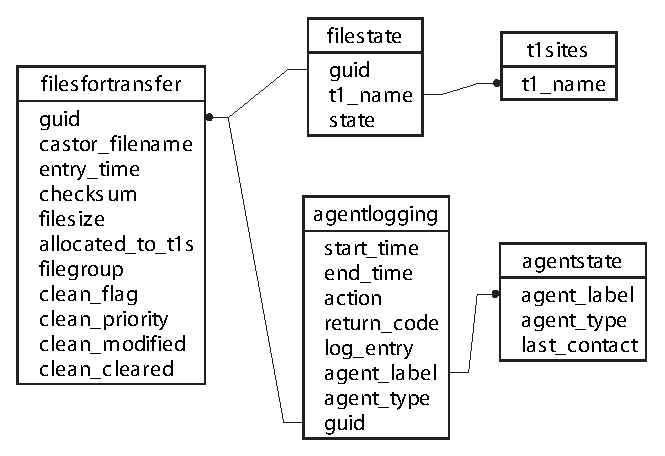
\includegraphics{v1_tmdb.eps}

\subsubsection{t1sites}
\begin{tabular}[tbp]{|c|c|c|c|}
\hline \multicolumn{4}{|c|}{t1sites}
\\ \hline field & type & constraints & index
\\ \hline t1\_name	& char(20) & primary key &
\\ \hline
\end{tabular}

{\bf t1sites} held the core list of T1s, to be used as a Foreign Key constraint on other tables. Sites in action at the start of DC04 were labelled as

\begin{tabular}[tbp]{|c|c|} 
\hline T1 & t1\_name
\\ \hline RAL & RAL		
\\ FNAL & FNAL
\\ IN2P3 & IN2P3
\\ PIC & PIC
\\ FZK & FZK
\\ \hline
\end{tabular}

�New� T1s could be added to this list if they contribute resources or if existing T1s change distribution scheme. This did not occur during DC04.

\subsubsection{filesfortransfer}
\begin{tabular}[tbp]{|c|c|c|c|}
\hline \multicolumn{4}{|c|}{filesfortransfer}
\\ \hline field & type & constraints & index
\\ \hline guid		&		char(36) &		primary key &
\\ castor\_filename	&	char(250) & &
\\ entry\_time		&	int & &
\\ checksum		&	int & &
\\ allocated\_to\_t1s	& char(1) & & x
\\ \hline
\end{tabular}

Guid indicates the unique identifier for a replica, and is of defined length. castor\_filename was the location of the file in Castor. The guid-Castor mapping will already be present in the LRC: it was also placed here to avoid extra LRC lookups. entry\_time was a unix timestamp (i.e. seconds since epoch start) of first entry into the distribution system. checksum was a normal unix checksum (generated with cksum). allocated\_to\_t1s indicated the state of the file (0 == true, !0 == false). false indicated files newly placed by Reco, true indicated that the configuration agent had allocated it to a number of T1s.

\subsubsection{filestate}
\begin{tabular}[tbp]{|c|c|c|c|}
\hline \multicolumn{4}{|c|}{filestate}
\\ \hline field & type & constraints & index
\\ \hline guid		&		char(36) &		primary key &
\\ t1\_name			& char(20)	& foreign primary &
\\ state			& int	& & x
\\ \hline
\end{tabular}

Guid again stored a unique file identifier, forming a primary key with t1\_name (a foreign key taken from t1sites). state indicated the current state of the propagation of the file. The following states were thought necessary: NEW, EB REALLOCATED, T1 REALLOCATED, IN BUFFER, AT T1, SAFE, CLEANED. During DC04, further states were added- some T1 specific, and some BAD states used for global management. Not all states were required, however- as failover was not tested in production, states EB and T1 REALLOCATED were not used.

The states were enumerated-

\begin{tabular}[tbp]{|c|c|} 
\hline index & state
\\ \hline 1	& NEW
\\ 2	& EB REALLOCATED
\\ 3	& T1 REALLOCATED
\\ 4	& IN BUFFER
\\ 5	& AT T1
\\ 6	& SAFE
\\ 7	& CLEANED
\\ 8+	& T1 specific
\\ \hline
\end{tabular}

% TODO: there were more states at the end than this!

as agents were the most frequent accessors of this information, and human operators accessed it via some front end which could interpret the state for them.

\subsubsection{agentstate}
\begin{tabular}[tbp]{|c|c|c|c|}
\hline \multicolumn{4}{|c|}{agentstate}
\\ \hline field & type & constraints & index
\\ \hline agent\_label		& char(20)	&	primary key &
\\ last\_contact	& 	int & &
\\ \hline
\end{tabular}

agent\_label was a text string that uniquely identified a distribution component-

\begin{tabular}[tbp]{|c|c|} 
\hline component & label
\\ \hline LCG SRM EB agent	& SE\_EB	
\\ GRID3 SRM EB agent	& SRM\_EB\_DCACHE
\\ SRB EB agent		& SRB\_EB
\\ RAL transfer agent	& RAL
\\ FNAL transfer agent	& FNAL
\\ IN2P3 trans. agent	& IN2P3
\\ PIC transfer agent	& PIC
\\ CERN transfer agent	& CERN
\\ FZK transfer agent	& FZK
\\ \hline
\end{tabular}

% TODO: There were more agents than this!

and was used as a foreign key for other tables. Agents were required to periodically make contact with the database by updating last\_contact. Any agent failing to update over the predefined period was considered to be unavailable

\subsubsection{agentlogging}
\begin{tabular}[tbp]{|c|c|c|c|}
\hline \multicolumn{4}{|c|}{agentlogging}
\\ \hline field & type & constraints & index
\\ \hline agent\_label		& char(20)	 & foreign &
\\ guid				& char(36)	 & foreign &
\\ start			& int & &
\\ end				& int & &
\\ action			& char(20) & &
\\ return\_code	 &	int & &
\\ log\_entry			& char(250) & &
\\ \hline
\end{tabular}

agent\_label was a unique agent label as described above; similarly, guid uniquely defined a file replica. start and end indicate the period over which the entry was relevant (i.e. for file transfer log entries). action contained one of a number of globally defined quick search entries (these were open for discussion/additions, but should definitely be globally agreed).

TRANSFER
Single entry per file transfer.

START
When agent starts.

FOUND
When agent checks transfer management tables and finds file entries to deal with (used during normal operations and recovery phase).

LEASED
When agent updates the agent state database.

FAIL
When agent needs to shut down (e.g. buffer has filled up, etc).

return\_code was used to store the return code of the operation that the log entry refers to. log\_entry provided a means to supply more descriptive entries if necessary.


\subsection{Overall process}
At the lowest level data sources added files to a general distribution buffer at CERN (on Castor stage disk), and placed a related POOL XML catalog fragment and checksum file in a dropbox to indicate the appearance of new files.

"Dropbox agents" processed new data, publishing GUID:PFN mappings to the LRC data to the TMDB with no associated state.

The transfer of data from CERN through one or more buffers to a number of Tier 1s was then be handled by a series of semi-autonomous agents. Each agent had certain limited responsibilities, including transferring files from one buffer to another, or cleaning a buffer when necessary.  In general agents were prohibited from contacting other agents (e.g. to check if the agent is working). The condition of agents at the next level was monitored in the TMDB (for the case of agents that are able to indicate their state) or be inferred from the fact that buffers are filling up (meaning that the next level agent is slow, or inactive and unable to indicate their state).

The first level of data distribution was a very simple replica manger named the "cionfiguration agent". This agent was the only agent aware of file-tier associations, and was the only one able to allocate files to T1s in the TMDB. 

Beyond this level agents were closely tied to specific distribution systems- e.g. SRB, gridFTP. Generically, however, they indicated whether files had been transferred to their buffer. Some agents in this chain indicated that files were fully safe- that they had been stored in MSS at a Tier 1. Other agents e.g. just staged data, making it available for other agents to pull. The latter process was used for all distribution schemes, with files being staged to export buffers dedicated to specific distribution schemes, and from then on to T1s.

\section{Experience}
Development was found to be straightforward, as only the messages to be passed
were defined: no new frameworks or coding languages were required. Around 50
agent instances were created, varying from a core set of 10. Each chain of
agents was coded and trivially tested within six weeks.

\subsection{Overall behaviour}
Typically files spent x amount of time "in distribution"- that is, between
being made available and being migrated by Castor when finally safe. Transfer 
rates of y, sustained over z were seen.

\subsection{The TMDB}
Performed very well, except when we did something (in retrospect) daft like
adding a new field to a table with a few hundred thousand entries in it. But
now we've seen what happens we can make a better version...

\subsection{RLS}
Good point was that it was used as a file and metadata catalogue for three
different distribution spaces, a use case not explicitly considered

The RLS was overloaded with queries early in the experiment: agent supervisors
noticed that (around the x) RLS queries slowed to the extent that the system
effectively locked up.

Basically due to number of parallel queries on RLS (numbers).

Other problems: slow access due to java single file-

Actions taken- bulk update where possible, move from java cli tools to C++ API.

Results...

\subsection{Dropbox agents}

\subsection{SRM chain}
The SRM chain showed that it was possible

\subsection{SRB chain}
The performance of the SRB chain was severely hampered by technical issues:
first with availability of the MCat metadata catalogue, hosted at RAL, and
secondly with a small number of bugs in SRB client and server, and Oracle
Linux implementations.

Did see transfer rates of ...

Shut down on ...

Ongoing investigations to determine causes of problems ...

\subsection{LCG chain}
The LCG chain exhibited the best performance of all the chains during DC04,
despite there not being a Storage Element export buffer available until
some time into the challenge.

\subsection{Real-time analysis agents}
Wow! 20 minutes lag before results available! :)

\section{Conclusions and future plans}
Gonna do it again, and it's gonna be better.

\begin{thebibliography}{9}

  \bibitem {FG96} {
  	Stan Franklin and Art Graesser,
  	\bf Is it an agent, or just a program? A taxonomy for autonmous agents},
    {\em Third International Workshop on Agent Theories, Architectures and Languages 1996, Springer-Verlag}.

  \bibitem {Setal03} {
  	M Aamir Shafi, Maria Riaz, Saad Kiani, Anjum Shehzad, Umer Farooq, Arshad Ali, Iosif C Legrand, Harvey B Newman,
  	\bf DIAMOnDS- Distributed agents for mobile and dynamic services},
    {\em Computing in High Energy Physics 2003 (CHEP03)}.

  \bibitem {B03} {
  	Joanna Bryson,
  	\bf Where should the complexity go? Cooperation in complex agents with minimal communication},
    {\em First International Workshop on Radical Agent Concepts 2003, Lecture Notes in Computer Science 2564
    }.

\end{thebibliography}
 
\end{document}
